\documentclass[a4paper,10pt]{report}
%\usepackage[T1]{fontenc} % on some systems T1 looks ugly
%\usepackage[cyr]{aeguill}
\usepackage[utf8]{inputenc} 
\usepackage{ucs} 
\usepackage{times} 
\usepackage{graphicx} 
\usepackage{makeidx}
\makeindex
%\usepackage{german}
\usepackage{color}
\pagestyle{empty}
\defä{\"a} \defÄ{\"A} \defü{\"u} \defÜ{\"U} \defö{\"o} \defÖ{\"O} \defß{\ss}
\addtolength{\topmargin}{-.5in}        % repairing LaTeX's huge margins...
\addtolength{\textheight}{1in}        % more margin hacking
\addtolength{\textwidth}{1.5in}
\addtolength{\oddsidemargin}{-0.75in}
\addtolength{\evensidemargin}{-0.75in}
\newcommand{\myspec}[1]{\textbf{\textit{#1}}}
\newcommand{\mytt}[1]{{\tt #1}}


% \usepackage[pdftex]{graphicx}
% \DeclareGraphicsExtensions{.png,.pdf,.jpg,.jpeg}
% \usepackage[pdftex,
% bookmarks=true,
% bookmarksnumbered=true,
% pdfpagemode=None,
% pdfstartview=FitH,
% pdfpagelayout=SinglePage,
% colorlinks=true,
% urlcolor=magenta,
% pdfborder={0 0 0}
% ]{hyperref}

%%%%%%%%%%%%%%%%%%%%%%%%%%%%%%%%%%%%%%%%%%%%%%%%%%%
%interesting settings for the page layout

%\setlength{\hoffset}{-18pt}
%\setlength{\oddsidemargin}{0pt}  % left margin, odd pages
%\setlength{\evensidemargin}{9pt}  % left margin, even pages
%\setlength{\marginparwidth}{54pt} 
%\setlength{\textwidth}{481pt}  % set the text width to about 17cm
%\setlength{\marginparsep}{7pt}
%\setlength{\topmargin}{0pt}  % no margin on top
%\setlength{\headheight}{13pt}
%\setlength{\headsep}{10pt} 
%\setlength{\footskip}{27pt}
%\setlength{\textheight}{700pt}

%%%%%%%%%%%%%%%%%%%%%%%%%%%%%%%%%%%%%%%%%%%%%%%%%%%
%% miscalleneous packages

% \usepackage[frenchb]{babel} % use this if you are French
% \usepackage{verbatim} % include eg: source code easily
% \usepackage[utf8]{inputenc} or \usepackage[latin1]{inputenc}

% If you are on Fedora Core you may have problems with accents
% in this case replace the accentuated characters like this :
%
%  é -> \'e
%  è -> \`e
%  ê -> \^e and so on
%
% To automate the replacement you can make yourself a script
% here is a handy command-line for doing this :
% perl -pi -e "s/é/\\\'e/g" main.tex

\usepackage{amsmath}
% math extension - one probably wants to use symbols like '[' (written as '$[$')
% or $\epsilon$

% see mymacros.sty - print nice chapter headers
%\usepackage{mymacros}

%%%%%%%%%%%%%%%%%%%%%%%%%%%%%%%%%%%%%%%%%%%%%%%%%%%

% headers and footers for your document
%\usepackage{fancyheadings}
\usepackage{fancyhdr}

% count the number of pages for display on footer
\usepackage{lastpage}

% width of the line for headers and footers
%\headrulewidth 0.5pt
%\footrulewidth 0.5pt
%\addtolength{\headwidth}{\marginparsep}

% uncomment the following lines for headers
% the following command need picture files : "logo-school.jpg" 
% and "logo-company.jpg" in the project directory
%
%        \lhead{\sl \includegraphics[height=1.1cm]{logo-school}}
%        \chead{}
%        \rhead{\sl \includegraphics[height=1.2cm]{logo-company}}


\usepackage{ucs}
\usepackage[utf8]{inputenc}


%%%%%%%%%%%%%%%%%%%%%%%%%%%%%%%%%%%%%%%%
%document headers and footers
\lhead{}
\chead{}
\rhead{}
\lfoot{TU-Clausthal}
\cfoot{\thepage/\pageref{LastPage}}
\rfoot{ \today } % -> \rfoot{\number\month/\number\day/\number\year} 
\pagestyle{fancyplain}



\title{{\bfseries\Huge
\hrulefill\\
\hrulefill CP-PAW\hrulefill\\
\hrulefill Coding Style Guide\hrulefill\\
\hrulefill\\}
\hfill\\
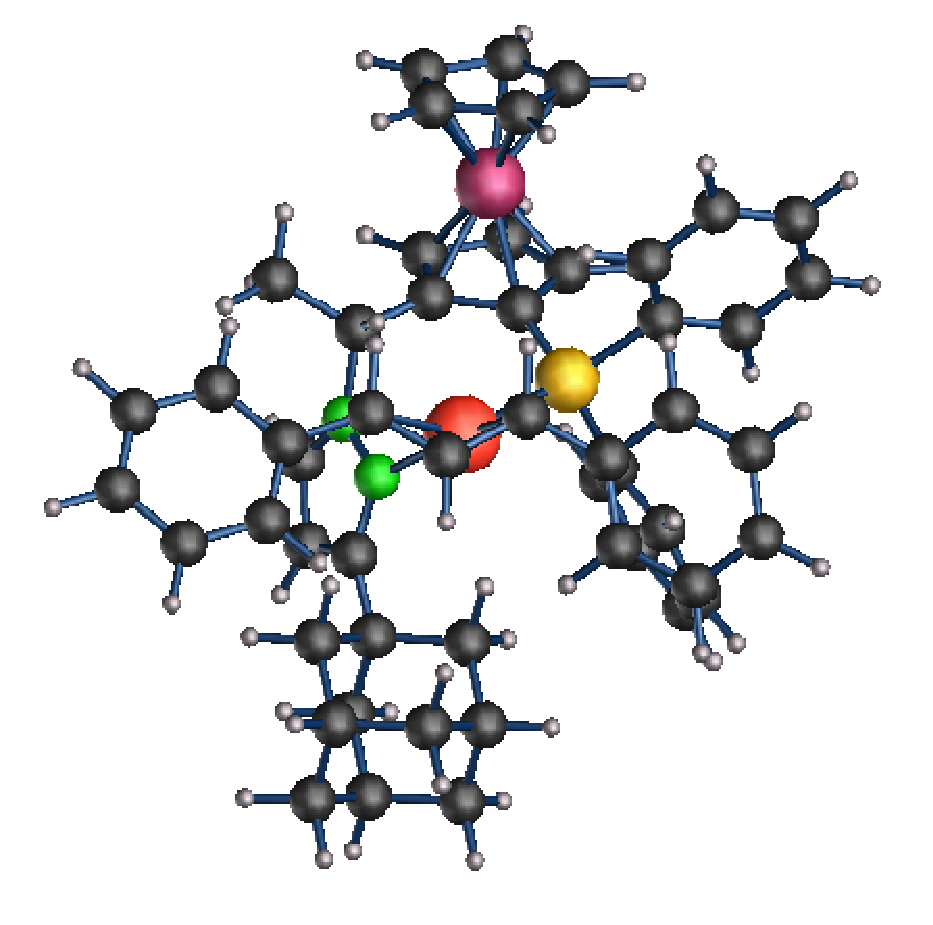
\includegraphics[width=9cm]{Figs/big.eps}
}
\date{\hrulefill\\Peter~E.~Bl\"ochl, Clausthal University of Technology\\(\today)}

\begin{document}
\maketitle

%======================================================
\section*{Preface}
%======================================================
In this document I will try to develop the coding styles that teh
CP-PAW code adheres to. It is meant to make the code more accessable
and it should also lay down a basis for joint development of the code.

Peter Bl\"ochl

\tableofcontents

%=======================================================================
\chapter{Coding design rules}
%=======================================================================
%
%====================================================================
\section{General coding design rules}
%====================================================================
%
%====================================================================
\subsection{Visual structure}
%====================================================================
An example for a subroutine is this \textit{``hello world''} routine.
{\small
\begin{verbatim}
!
!     ...1.........2.........3.........4.........5.........6.........7.........8
      SUBROUTINE HELLOWORLD(NFIL)
!     **************************************************************************
!     **  WRITES HELLO WORLD TO A FILE                                        **
!     **************************************************************************
      IMPLICIT NONE
      INTEGER(4)  ,INTENT(IN) :: NFIL     ! FORTRAN UNIT
      CHARACTER(8)            :: HELLOWORLD
!     **************************************************************************
!
!     ==========================================================================
!     ==  define                                                              ==
!     ==========================================================================
      HELLOWORLD='HELLO WORLD!'
!
!     ==========================================================================
!     ==  WRITE HELLOW WORLD                                                  ==
!     ==========================================================================
      WRITE(NFIL,FMT='(A)')HELLOWORLD
      RETURN 
      END
\end{verbatim}}

\begin{itemize}
\item   I am using lines with 80 characters wide, because this size is still
  easily printed without breaking lines. Therefore, I begin coding
  creating a ruler, 
{\small
\begin{verbatim}
12345678901234567890123456789012345678901234567890123456789012345678901234567890
!     ...1.........2.........3.........4.........5.........6.........7.........8
\end{verbatim}} 
  which also serves a header line for each
  subroutine.  The first line with the numbers only serves to construct
  the actual header line below. Then it is deleted.

\item All comment lines will have the same length so that the width is always 
available during coding.

\item Subroutine documentation follows directly the calling sequence and have the form
{\small
\begin{verbatim}
!     **************************************************************************
!     **  this is a comment                                                   **
!     **************************************************************************
\end{verbatim}}
The variable declaration is finished by another stared line.

\item Comments are that describe a task are denoted as
{\small
\begin{verbatim}
!      =========================================================================
!      ==  this is a comment                                                  ==
!      =========================================================================
\end{verbatim}}

\item One line comments that refer only to the next one or two lines
can have the form
{\small
\begin{verbatim}
!      == this is a comment ====================================================
!      __this is a comment______________________________________________________
\end{verbatim}}
\end{itemize}
%
%====================================================================
\subsubsection{Indentation}
%====================================================================
\begin{itemize}
\item We begin a code line always on column 7 as in fortran77 and try to
stop whenever possible on or before column 80. The motivation is that
code used for debugging can be inserted starting in the first line, so
that corruptions of the code are immediately obvious.

\item \texttt{DO} loops and and \texttt{IF} statements are indented by two
characters for each level. This is a compromise between visibility on
the one hand and on the other hand the space requirements for
commands.

\item Continuation lines are indicated by an \texttt{\&} at the end of the
continued line as required by the the fortran90 standard and by
another \texttt{\&} in column 6 of the continued line. In Fortran 90
the first \textit{\&} in the continuation line is not required, but it
enhances clarity if the code structues.
\end{itemize}

%
%====================================================================
\subsection{Declarations}
%====================================================================
\begin{itemize}
\item All variables are declared explicitely, hence we introduce an
\texttt{IMPLICIT NONE}.

\item Input and output variables are explicitely declared with
\texttt{INTENT(IN)}, \texttt{INTENT(OUT)}, and
\texttt{INTENT(INOUT)}. \texttt{INTENT(INOUT)} is avoided whenever
possible, and it is never used, when the more specific statements are
used.

\item The dimension is never declared with the statement
$\texttt{DIMENSION}$, bcause this is too bulky.
Thus we use
{\small
\begin{verbatim}
REAL(8) :: x(10)
\end{verbatim}}
instead of
{\small
\begin{verbatim}
REAL(8),dimension(10) :: x
\end{verbatim}}

\item   With the exception of do-loop variables or closely related
  variables, each variable is specified on one line, and, whenever
  suitable, followed by a comment explaining it.  {\small
\begin{verbatim}
REAL(8) :: x(10)  ! coordinate array
\end{verbatim}}

  \item currently the default sizes are
    \texttt{LOGICAL(4),INTEGER(4),REAL(8),COMPLEX(8)}. This is a
    compromize between being specific, and compatibility with 32-bit
    and 64-bit processors. (In future we may switch the
    \texttt{INTEGER(8)} or default integer, \texttt{INTEGER}, but this
    must be done consistently throughout the complete code.)

\end{itemize}


%=======================================================================
\chapter{Object-oriented programming}
%=======================================================================
The main idea of object-oriented programming is to structure the code
in terms of rather independent agents, also called objects. An agent
consists of a set of functions (operations) and the memory needed to
perform these functions. Thus a higher level language is constructed,
which essentially calls these agents and controls the communication
between them. On the higher level the operations can be combined again
into agents creating an even higher level language. This approach is
scalable in complexity, and allows to efficiently develop and maintain
large codes.

The agents need to be prepared as logical entities. What this means is
rarely clear and a good code is characterized by a good choice of
agents. Some design rules are important: 
\begin{itemize}
\item The same data should not be dublicated in different agents. This
is not always possible, and if it is not one should at least identify
one agent who is responsible for a certain variable. Otherwise the
value of that data may become unsynchronized.
\item The amount of external information required by an agent 
to perform its function, should be minimized.
\item The agents and functions should be intuitive. 
\end{itemize}


%
%====================================================================
\section{Encapsulation}
%====================================================================
The  design  of  an  object  distinguishes  clearly  between  what  is
accessable  towards  the  outside  of  the  object  and  the  internal
operations of the  object. The latter should be  made invisible to the
user. This concept is called  \textit{encapsulation} and is one of the
main concepts of object oriented programming.

An object contains two sets of subroutines: those that are available
to the user of the object and those that are required used only by
other routines of the object. To make this evident I introduced the
following naming convention.
\begin{itemize}
\item \textit{objectname}\texttt{\$}\textit{functionname} is a
  subroutine that can be accessed from the outside
\item \textit{objectname}\texttt{\_}\textit{functionname} is a
  subroutine that can be only from inside the object.
\item \textit{objectname}\texttt{\$\_module} or
  \textit{objectname}\texttt{\$\_interface} is the module of the
  object. The module contains the permanent data of the object,
  declarations of common data structures and the like. At the moment
  there is no clear distinction between internal and external module
  files. Type declarations, definition of overloaded operations may
  need to be communicated to the outer world, while the internal data
  should be accessable only by calling subroutines of the object.
\end{itemize}



%
%====================================================================
\section{Design of a general object}
%====================================================================
An Object consists of a module holding general data and a set of
functions (subroutines).  The module holding general data is named
\texttt{OBJECT\_MODULE}, where \texttt{OBJECT} stands is a place
holder of the object name.

The functions of teh object can be public and private. The public
functions can be accessed from everywhere, which the private functions
must only be called from within the object. The public functions are
named \texttt{OBJECT\$FUNCTION} and the private functions are named
\texttt{OBJECT\_FUNCTION}, where \texttt{FUNCTION} is a place holder
for the function name.

Data will be exchanged with the object via functions 
\begin{verbatim}
OBJECT$GETCH(ID,VAL)      ! STRINGS
OBJECT$GETL4(ID,VAL)      ! LOGICAL SCALARS
OBJECT$GETI4(ID,VAL)      ! INTEGER SCALARS
OBJECT$GETR8(ID,VAL)      ! REAL SCALARS
OBJECT$GETC8(ID,VAL)      ! COMPLEX SCALARS
OBJECT$GETI4A(ID,LEN,VAL) ! INTEGER ARRAYS
OBJECT$GETR8A(ID,LEN,VAL) ! REAL ARRAYS
OBJECT$GETC8A(ID,LEN,VAL) ! COMPLEX ARRAYS
\end{verbatim}
There is a similar set of functions where \texttt{GET} is replaced by
\texttt{SET}.  \texttt{ID} is an character identifier, which is checked
and \texttt{LEN} is the size of the array. The length is explicitely
checked for the \texttt{OBJECT\$GET..} functions. For the set
functions the length may be used to set a variable determining the
size, but it is tested if this size variable has not been set
otherwise.

It is sometimes neccesary to make function interfaces publically
available, for example for generic subroutine names. In this case a
second module with name \texttt{OBJECT\$INTERFACE} is created.
%
%====================================================================
\section{Design of a dynamical object}
%====================================================================
The basic iteration is done by three functions
\begin{verbatim}
OBJECT$ETOT()
OBJECT$PROPAGATE()
OBJECT$SWITCH()
\end{verbatim}

Usually the object has to set itself up before the iteration can
begin. This is done by a public function
\begin{verbatim}
OBJECT$INITIALIZE()
\end{verbatim}
Such a function is provided if internal data need to be made available
externally. Preferred is an internal function
\texttt{OBJECT\_INITIALIZE()}, that is called whenever needed as
decided by an internal flag \texttt{TINI} of type logical.

For reading and writing the data to a restart file the functions
\begin{verbatim}
OBJECT$READ(NFIL,NFILO,TCHK)
OBJECT$WRITE(NFIL,NFILO,TCHK)
\end{verbatim}
are provided.

The setting of the object is reported by the function
\begin{verbatim}
OBJECT$REPORT(NFIL)
\end{verbatim}

The object has a number of parameters that allow to control its
functionality.
\begin{itemize}
\item \texttt{STOP}; logical; sets initial velocities to zero.
\item \texttt{DT}; real; timestep
\item \texttt{FRICTION}; real; friction parameter $\alpha\Delta/2$
\end{itemize}   

\begin{itemize}
\item \texttt{ekin}; kinetic energy
\item \texttt{epot}; potential energy
\item \texttt{force}; generalized force, $-\frac{dE}{dx}$
\item \texttt{xp}
\end{itemize}   

\printindex
\end{document}


